% !TEX root = ./paper.tex

In this section, we evaluate \tcpls using two different types of experiments.
First, we analyze the raw performance of our \tcpls prototype and how \tcpls interacts with middleboxes in a controlled environment. We then emulate, using Mininet~\cite{handigol2012reproducible}, more complex scenarios including failover and multipathing.


%Our objective is to evaluate whether our design and implementation are indeed
%fast, flexible and does not conflict with several commercial and open-source
%middleboxes. Moreover, we expect to showcase and compare TCPLS's functionalities
%such as the App-level connection migration, the failover mechanism or the
%bandwidth aggregation capability. We discuss them against the state
%of the art designs, such as mvfst~\cite{mvfast}, quicly~\cite{quicly},
%msquic~\cite{msquic}, MPTCP~\ref{mptcp}, pquic~\cite{pquic},
%quic-go~\cite{quic-go} and MPQUIC~\ref{mpquic}.

%TODO do we also evelatuate security? with a simple proof and discussion?

%To evaluate \tcpls's functionalities, we rely on reproducible network
%experimentations with Mininet~\cite{mininet}. Our objective is to compare the
%behaviour of \tcpls with the state of the art, and to make it easily
%reproducible for future works, as the quic implementations continue to evolve.


\subsection{Raw Performance} \label{sec:perf}

To evaluate the raw performance (Sec.~\ref{sec:perf}) and middlebox traversal
(Sec.~\ref{sec:middlebox}) of our \tcpls prototype, we use the testbed depicted in Fig.~\ref{fig:perf_testbed}. Our testbed is made of three servers equipped with Intel Xeon CPU E5-2630 2.40GHz, 16 threads, at least 16~GB RAM, running Debian with Linux 5.9 and 5.7 kernels. Two of these machines are used as, respectively, Client and Server, while the third one is used as a router or a middlebox, depending on the scenario. Each machine is equipped with an Intel XL710 2x40Gbps NIC. With jumbo frames, a single \tcp connection can saturate the 40~Gbps path. With a 1500 bytes MTU, a single connection reaches 22~Gbps.

\begin{figure}[!t]
  \begin{center}
    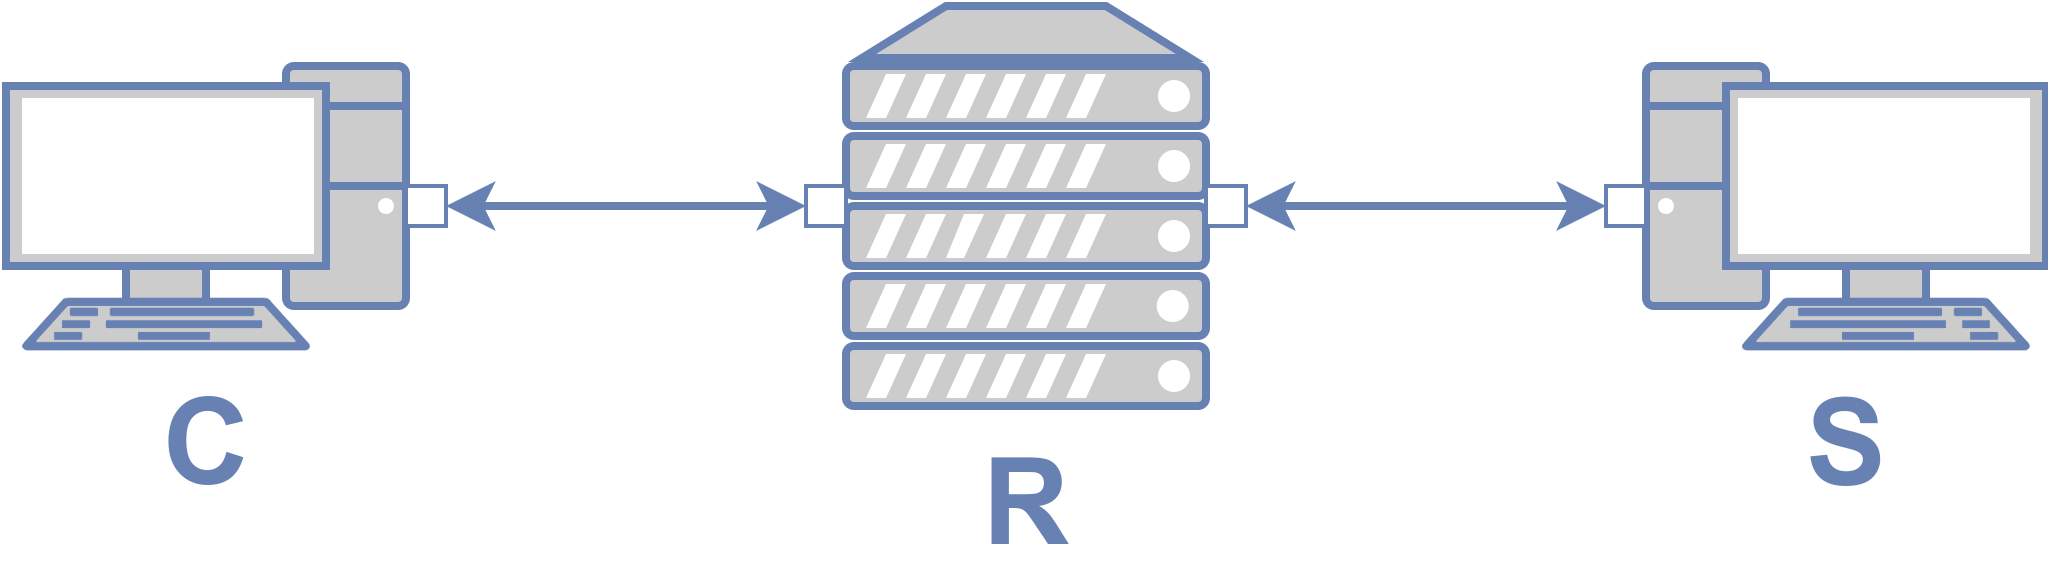
\includegraphics[width=.6\columnwidth]{figures/testbed.png}
  \end{center}
  \vspace{-0.5cm}
  \caption{Performance Measurements Setup. C = Client. S = Server. R = Router/Middlebox.}
  \label{fig:perf_testbed}
\end{figure}


The first question we want to answer is whether \tcpls can compete with the
traditionnal \tls over \tcp stack. We also compare our \tcpls prototype with
different \quic implementations.

\paragraph*{\tcpls}
For all the \tcpls measurements, we use a custom application that performs
large memory-to-memory transfers over a \tcpls session using a single stream.
\tcpls is configured to use the AES128-GCM-SHA256 cipher. Fig.~\ref{fig:perf} provides the goodput as measured in our testbed. We report both the bandwidth in megabits per second and packets per second. Each bar in Fig.~\ref{fig:perf} corresponds to the median measured over 10 seconds of stable throughput. The bottom bar (labeled ``\tcpls tso on mtu 900'') is the highest median goodput that we measured with \tcpls: 12.4~Gbps. This result was obtained with jumbo frames (i.e. ,9000 bytes MTU) and using \tcp Segmentation Offload (TSO) on the NICs. TSO is a standard feature that is enabled by all high-speed NICS. This result is impressive given that we measure that AES128-GCM-SHA256 peaks at 13.1~Gbps when doing in-memory encrytion/decryption on our testbed's servers.
The next bar (labeled ``\tcpls tso on'') shows that with TSO and a standard frame size (1,500 bytes MTU), the goodput still reaches 10.84 Gbps. These
results should be compared with the 22~Gbps \tcp reaches in the same
environment using \texttt{iperf} but without any encryption.


%the shows several interesting results. First, while offering similar (and more)
%capabilities than what QUIC is providing today,
%\tcpls is also more than twice faster than the strongest evaluated QUIC
%implementation (quicly) over CPU limited experimentations. We evaluate \tcpls

We also compared \tcpls's native bandwidth aggregation using two streams with a
single stream produced by our \tcpls client on the top of the \mptcp kernel
creating two \mptcp subflows. Our \tcpls scheduler is a simple round-robin. The
\mptcp scheduler is the lowest-RTT scheduler enabled by default. Both
measurements are taken over the same 0.94.7 \mptcp kernel with a path MTU of
1,500, in which \mptcp is disabled when the \tcpls native experiment is
performed.  Surprisingly, \tcpls's native bandwidth aggregation outperforms
\mptcp. Both experiments are CPU limited, and suffers from a raw throughput
degradation compared to the single-path experiment. \tcpls's reordering is
implemented with an efficient heap~\cite{heap-github} highly efficient in
resizing, and pushing unordered records
in $O(log(n))$ for $n$ elements in the heap, and retrieving ordered records in
$O(1)$. Besides \tcpls's native  multipath uses the \tcp optimized stack, which
together offer a strong secure bandwidth aggregation solution.

We then evaluate the impact of adding the \tcpls-level acknowledgements
described in Sec.~\ref{failover} to support failover.
% Thanks to these acknowledgements, \tcpls can support failover.
From a performance viewpoint, they increase the number of control records and
the number of system calls. Our prototype currently sends a \tcpls-ack for every
16 received records. Our measurements indicate that with this functionnality,
\tcpls reaches 9.65 Gbps with a $1500$ bytes MTU.


\begin{figure}[!t]
  \begin{center}
    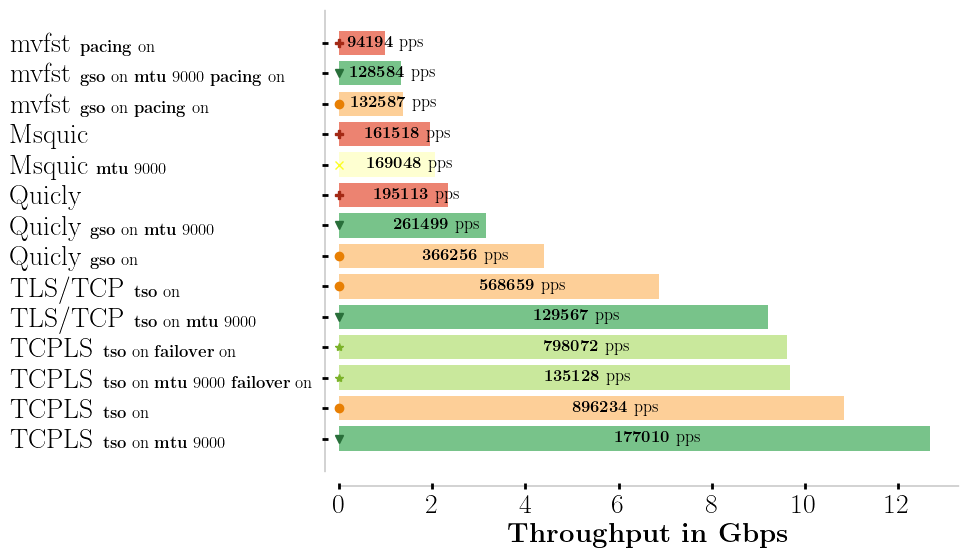
\includegraphics[width=\columnwidth]{figures/perf_analysis.png}
  \end{center}
\vspace{-0.5cm}
  \caption{\tcpls raw performance and comparison with state of the art.  The \tcpls prototype is faster than \tls over \tcp and different \quic implementations.}
  \label{fig:perf}
\end{figure}


%in four different settings: with a path mtu of 1500 or 9000, and with failover
%enabled or not. The failover functionality is an internal stack feature that
%provides session reliability, which increases the number of syscalls that TCPLS
%makes by exchanging TCPLS-level record acknowledgments. We currently send an
%ac%k for throughput at the price of a slower recovery in case of network
%failure.

\paragraph*{\tcpls vs. \tls/\tcp} We now compare the performance of \tcpls with
the traditional \tls over \tcp stack. To have a fair comparison, we use
\texttt{picotls}'s perf client/server implementation with the same commit as our initial fork for \tcpls. Fig.~\ref{fig:perf} shows that \tls/\tcp provides a lower performance than \tcpls with regular and jumbo frames. This can be explained by the receiving buffer size provided to \texttt{read()}, which is hardcoded to 16,384 bytes in \texttt{picotls}'s perf client. This implementation choice results in fragmentation on the receiver and prevents it from using the zero-copy code path provided by the library. \tcpls uses a larger read buffer and benefits from zero-copy. At first, one may consider this as an unfair comparison, however the devil is in the details. In our \tcpls implementation, the application developers cannot touch \texttt{read()}'s interface. This implies that an application developer cannot missuse the relationship between \tls and \tcp by creating fragmented records and doing unecessary copies to handle those fragments. \tcpls's design and implementation try to prevent fragmentation by, first, having a sufficiently large read buffer size. Second, \tcpls only starts deciphering a record when it has received the entire content. \tls/\tcp record fragmentation is provided by \tls libraries as a usability feature that spares the application developers from taking into account all \tls details, at the cost of lower performance. With \tcpls, application developers can ignore \tls details without missusing the interface, which is the reason why this comparison is interesting. \tcpls constrains the application developer to use the buffer type provided by the API, but offers zero-copy deciphered records in return.

%\todo{OB: pas sur que la suite est nécessaire} Moreover, but this has not
%yet been implemented, it could be interesting to match the TLS record size to
%the congestion window to deliver faster the data to the application when the
%network is congested.

\paragraph{\tcpls vs. \quic}
Although \quic~\cite{draft-ietf-quic-transport} is a young protocol, there are
already more than a dozen implementations~\cite{marx2020same,quicimplem,yang2020making} under active
development. We compiled and installed three representative \quic implementations in our testbed: Facebook's \mvfst~\cite{mvfst-github,Joras_mvfst}, Microsoft's \msquic~\cite{msquic-github}, and Fastly's
\quicly~\cite{quicly-github}. They are all developed by large companies that (plan to) use them in production and include their own benchmarking application to perform throughput measurements. Furthermore, \mvfst and \quicly support Generic Segmentation Offload (GSO), that should improve performance by offloading \udp segmentation and checksum computation to our NICs. We use the
implementation's bechmarking application as is, exploiting the optional
arguments provided by their interface to increase the throughput but drawing the
line there. That is, we do not modify the \quic implementations and use their default cipher. Note that, we tried to match the transport parameters to the same ones used by \tcpls when they did not adversaly affect \quic's performance too much. For example, several congestion control algorithms are implemented in the different \quic stacks, but setting a different one than the suggested default led to lower performance or unstable throughput measurements.

The results shown in Fig.~\ref{fig:perf} show that \tcpls compares favorably
with the tested \quic implementations. The fastest \quic implementation is
\quicly. Thanks to GSO, it reaches 4.4~Gbps in our testbed with a 1,500 bytes
MTU. This result is directly comparable to \tcpls with TSO enabled, which still
performs more than twice faster at 100\% CPU peak with similar configurations
for the receiving buffer size. Suprisingly, \quicly's performance decreases with
jumbo frames but is still faster than when GSO is disabled.
\msquic could only reach 1.96~Gbps and \mvfst was slower despite GSO.


%QUIC is young protocol, and all implementations are in active development, with
%different states for their available features and optimizations. For example,
%none of the implementations were able to take advantage of a path mtu larger
%than 1500, and it even degraded the performance in the case of quicly. Two of them
%(quicly and mvfst) have implemented the support for \texttt{gso} leading in the
%case of quicly to more than 4 gb/s of throughput with a udp payload length
%configured to match TCP (1460).


%We perform a throughput evaluation of \tcpls and compare it to several major
%QUIC implementations: mvfst~\cite{} from Facebook, msquic~\cite{} from Microsoft
%and quicly~\cite{} from Fastly. Our choice of QUIC implementations was mainly
%influenced by the availability of a client/server perf tool specifically
%engineered for a throughput evaluation. A second criterion was the advancement
%of the implementation and the quality of the code. We hope to avoid most of the
%bugs negatively impacting their results by selecting the QUIC implementation
%that show advanced features and testings. A third criterion was the development
%language used. \tcpls is written in C, and we prefer to compare it against QUIC
%implementation written in a language compiled by clang or gcc. Mvfst, msquic
%and quicly meet these criteria.


\subsection{Middlebox Interference}
\label{sec:middlebox}

A full evaluation of middlebox interference would require measurements in various operational networks that include such devices~\cite{honda2011still,raman2020measuring,o2016tls}. This is
outside the scope of this paper and left for further work. Nevertheless, we have tested \tcpls against different opensource and commercial stateful
firewalls and proxy implementations (i.e., pfSense, IPFire, Cisco ASAv,
mitmproxy) and found no unexpected interference. Stateful filtering and stateful
packet inspection policies did not impact connectivity, and transparent TLS proxy successfully triggered \tcpls fallback to \tls/\tcp. Still, the security
appliances that block \tls 1.3 or some of its features
\cite{lee2019matls,Bock_China,raman2020measuring} would also block \tcpls.
%pervasive monitoring allows for configurable TLS extensions blocking
%\cite{rfc7258}. This is handled properly by \tcpls fallback mechanism.

When faced with middleboxes that intercept \tls 1.3~\cite{Bock_China,raman2020measuring}, we need to consider the \tcpls handshake \tls extensions: \tcpls, \join, SESSID, and COOKIE. The other
\tcpls messages through the Secure Control Channel are indistinguishable from
classical \tls records (i.e., they look like encrypted application data
for the middlebox). If a clients attempts to open a \tcpls session
through a \tls termination proxy, it sends a \textsc{ClientHello} with the
\tcpls extension. If the proxy does not support \tcpls, it replies with a
\textsc{ServerHello} message that does not include the \tcpls extension. From
this point, the client implicitely falls back to \tls, and continues with the
handshake.

Certain legacy \tls server implementations are known not to implement the \tls
specification properly and might abort connections when receiving unknown \tls
extensions. Analogous behavior has been observed in overly restrictive stateful
firewalls. To ensure connectivity in the presence of such policies, \tcpls
implements an explicit fallback mechanism. If a client receives a \tcp \rst in
response to the \tcpls \textsc{ClientHello}, or no response, it
tries negotiating a regular \tls connection, either
immediately or after a timeout. Similarly, a \tcpls \join extension might be
blocked on a path. In this case, the subflow attachment is canceled, and
the application is directly notified to be able to react appropriatly (e.g.,
to cancel a migration attempt).

%We tested \tcpls against opensource and commercial stateful firewalls and proxy
%implementations and (i.e., pfSense, IPFire, Cisco ASAv, mitmproxy) and found no
%interferences. Still, certain middlebox security appliances that implement
%pervasive monitoring allows for configurable TLS extensions blocking
%\cite{rfc7258}. This is handled properly by \tcpls fallback mechanism.


\subsection{Bandwidth Aggregation}
\label{sec:bwaggr}
We compare the \tcpls bandwidth aggregation capability to the state-of-the-art
\mptcp. To this end, we build a Mininet network~\cite{handigol2012reproducible}
composed of a client and a server, both dual-stacks. The IPv4 and IPv6 paths are completely disjoint in this emulated network. Both protocols run in the same Mininet topology with two IP paths available, each offering 25Mbps and 10ms latency. The experiment consists in transfering a 60MB file over a single path and then enabling the second one after $5$ seconds. \mptcp automatically detects the new path once we enable the second network interface
on the Client. For \tcpls, managing paths is easier: the application can use the API to add local or peer-related addresses at any point of the session. In this experiment, we send this information at $5$ seconds, create a new \tcp connection to the peer, and attach a new stream to this new connection. Our results appear in Fig.~\ref{fig:multipath_aggregation}. Both stacks aggregate the two paths and reach a goodput of $\approx$ 50 Mbps. There are two major differences between the two stacks. First, when a new network interface comes up, the Linux kernel takes some time to configure its IP address, to add the required routes, and to finally inform \mptcp~\cite{paasch2012exploring}.
This explains the time that \mptcp needs to start to use the new path.
Second, \tcpls's aggregated goodput seems less stable than \mptcp. We may explain this discrepancy by the difference of chunk size manipulated by the reordering algorithm: \mptcp reorders packets with a payload of 1,460 bytes, while \tcpls in this experiment reorders records with the maximum payload size of 16,384 bytes. That means that \tcpls, upon unordered records, would need to reorder and deliver much larger chunks of data, leading to larger goodput irregularities than \mptcp. However, \tcpls might negotiate the record size to smooth out this irregularity. Setting a record size around 1,500 bytes would make \mptcp and \tcpls' results lookalike, but would be slightly more CPU costly since we need to use the encryption/decryption code path more often.
Appendix~\ref{appendix:aggr} shows the results of the same experiment but using
a \tls record size of 1,500 bytes instead.

\begin{figure}[!t]
  \begin{center}
    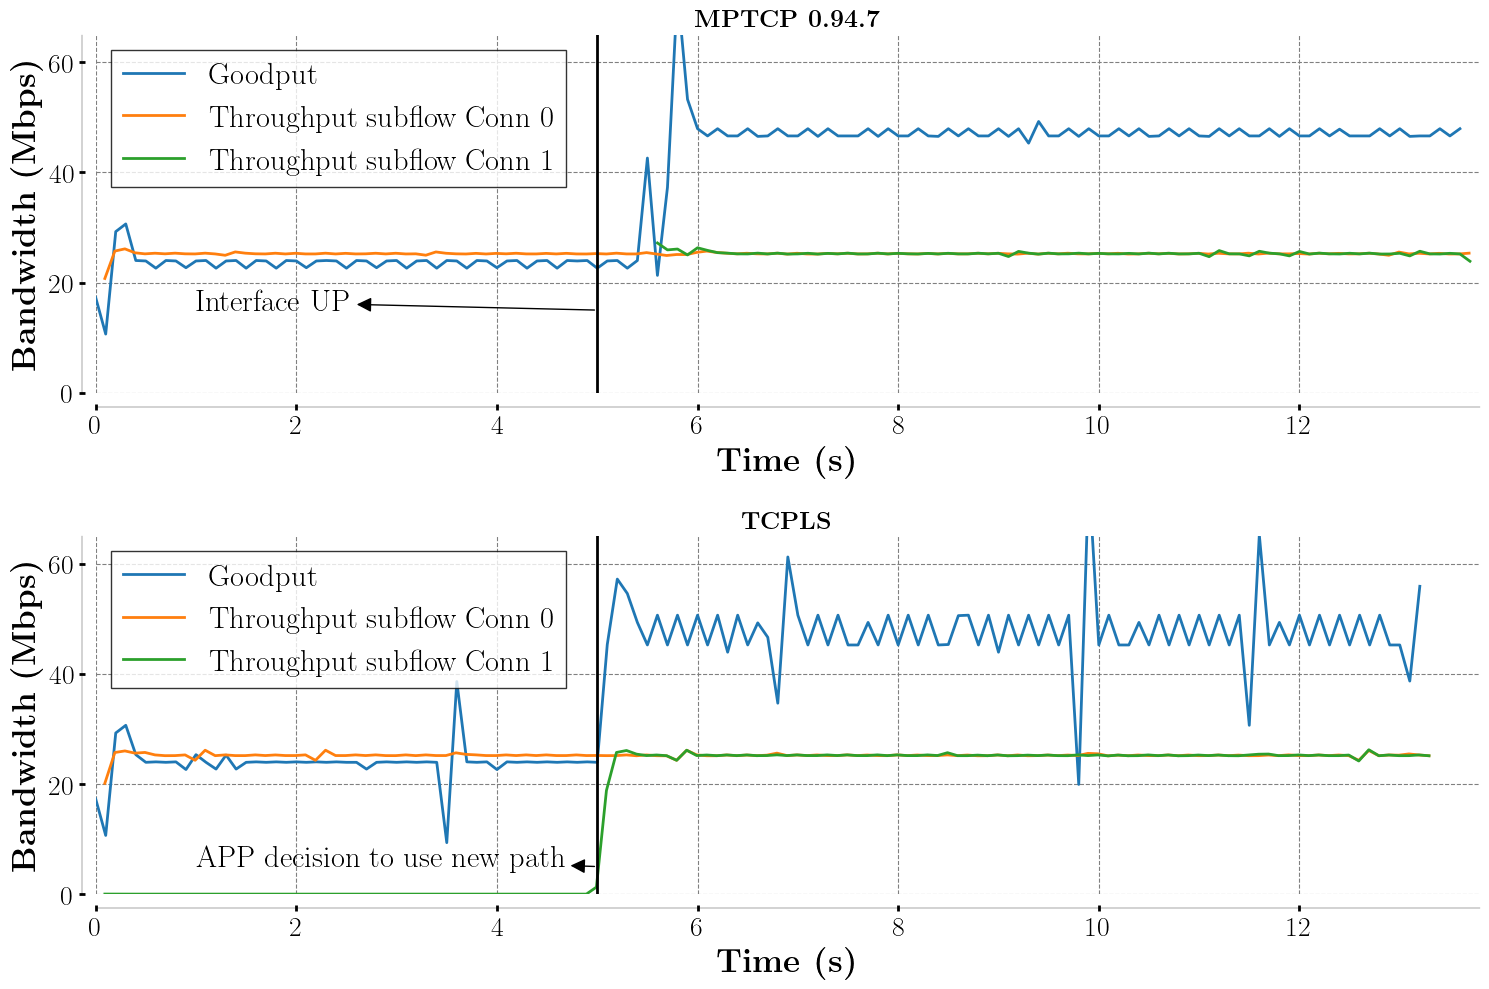
\includegraphics[width=\columnwidth]{figures/aggregate_dual.png}
  \end{center}
\vspace{-0.5cm}
  \caption{Bandwidth aggregation comparison between \mptcp (top plot) and
    \tcpls (bottom plot) with a record payload size of 16,384 bytes.}
  \label{fig:multipath_aggregation}
\end{figure}

\subsection{Failover}
\label{sec:eval_failover}

The failover feature is designed to provide resilience to \tcpls connection
failures. From middlebox interference to mobile client loosing
their connection to the access point (LTE or Wi-Fi), network outages may happen
for various reasons. We first discuss and compare the recovery speed
after a network outage, for different types of outages. Fig.~\ref{fig:recovery}
compares the goodput achieved by both \mptcp and \tcpls when they suffer an
outage on their main path and fallback to their secondary path. Both the client and the server are configured with two interfaces, with one of them set to the backup mode in the case of \mptcp (no connections are made to the backup interface unless an issue is detected on the first path). We consider three types of outages: a middlebox blackholing all the traffic, the reception of a spurious \rst, and the loss of the interface for \mptcp.

\begin{figure}[!t]
  \begin{center}
    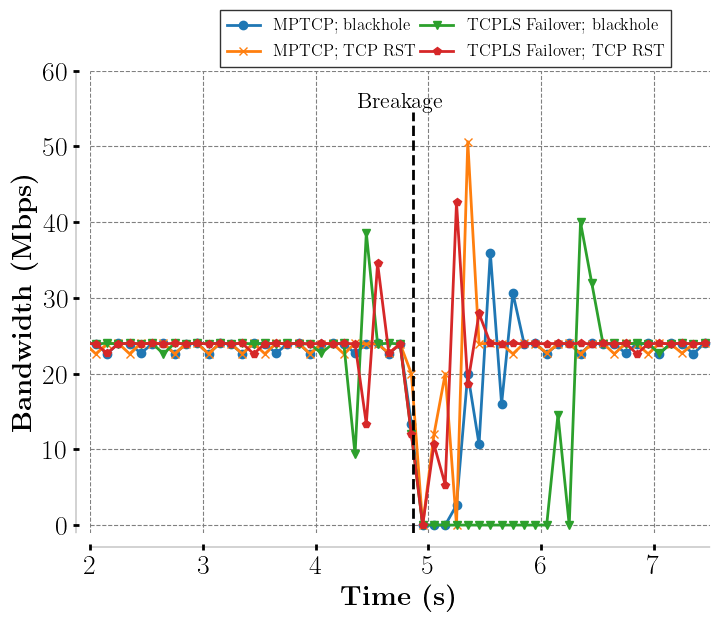
\includegraphics[width=.8\columnwidth]{figures/breakage_analysis.png}
  \end{center}
\vspace{-0.5cm}
  \caption{Recovery delay analysis.}
  \label{fig:recovery}
\end{figure}

Our results show different behaviours: upon reception of a \rst, both
\tcpls and \mptcp react fast. A network outage
is more difficult to handle: both stacks rely on timers and base their
decision to switch the path on their expiration. In the case of \tcpls, we
configure a timer using the $TCP\_USER\_TIMEOUT$ \tcp option. The scenario is as
follows: when the server enables failover, it sends a $USER\_TIMEOUT$ to protect the transfer. This option is sent through the secure control channel to indicate to the client \tcpls's stack that it should not wait more than $X ms$ between successful reads of data, with $X$ a parameter of this option. For this experiment, the $USER\_TIMEOUT$ is set to $250~ms$. When the timer expires, \tcpls creates a connection over the other path and joins the session. It then replays the unacknowledged records. Once these steps have succeeded, the transfer can continue. In our experiments, it took around $\approx 1$ second to recover from the outage.


\begin{figure}[!t]
  \begin{center}
    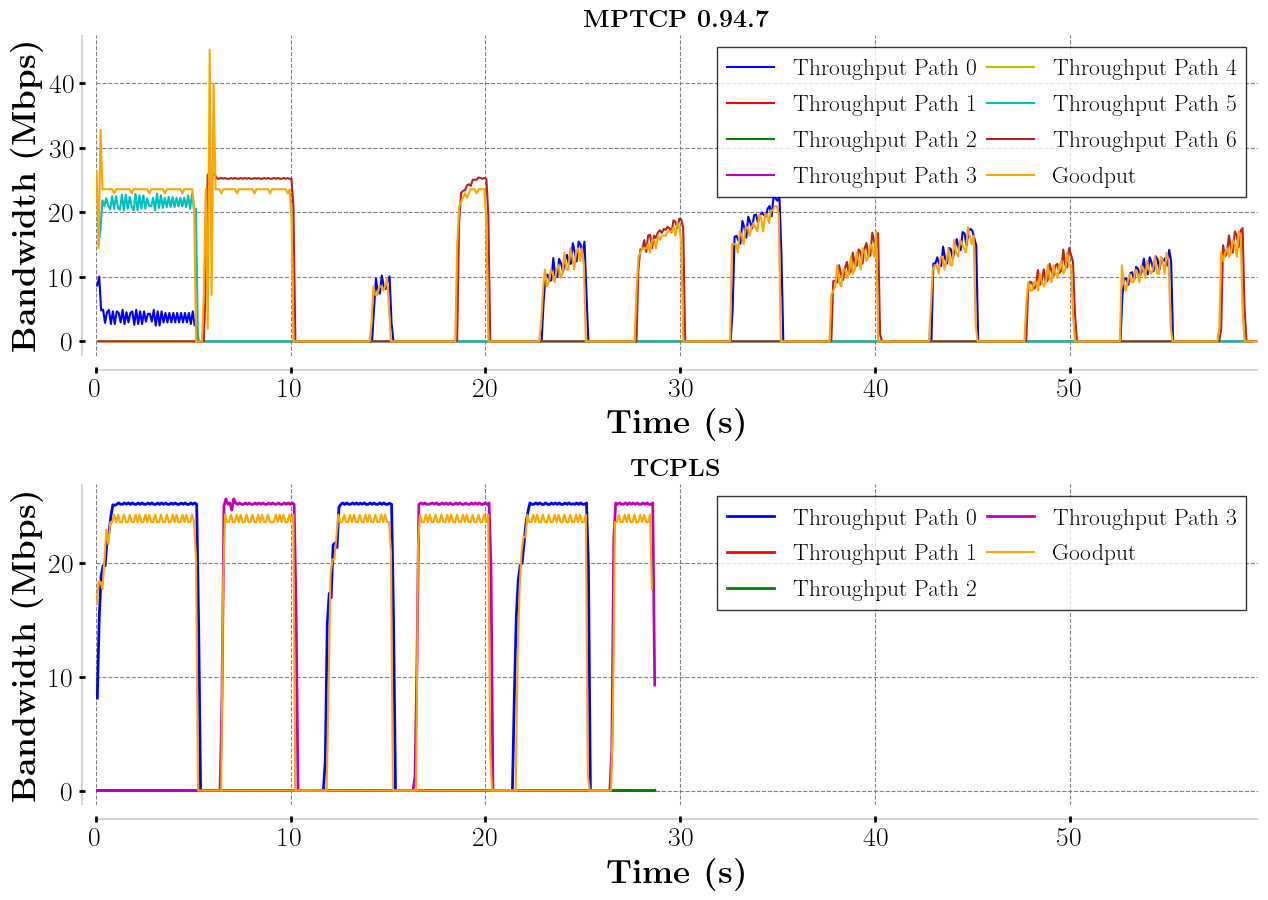
\includegraphics[width=\columnwidth]{figures/tcpls_mptcp.png}
  \end{center}
\vspace{-0.5cm}
  \caption{\mptcp has difficulties to react to successive network outages. \tcpls reacts quickly to such outages.}
  \label{fig:failover}
\end{figure}

The second experiment consists in observing how different multipath
implementations behave when several failures occur during a data transfer. We
tested several multipath implementations: \mptcp, PQUIC with the multipath
plugin~\cite{de2019pluginizing}, and MPQUIC~\cite{de2017multipath}.
The results with PQUIC and MPQUIC were disappointing. We dug into these implementations and observed that they were not programmed to detect network failures and correctly switch the network path, thus we preferred to ignore those results. \mptcp has a longer development background and is used in production and maintained. Fig.~\ref{fig:failover} shows how \mptcp and \tcpls perform when three paths out of four are blackholled every five seconds. The protocol has first to find the healthy path and recover the session over it. We observe that \mptcp's default path manager performs well on the first
failure. For the next ones, it seems to require several seconds to
recover the right path. Besides, \mptcp seems to remember that something wrong happened, and enters a kind of congestion avoidance state until the end of the transfer. We may question this design choice, since many \tcp connections on the Internet have a shorter lifespan than 10 seconds (i.e., the time after which \mptcp should re-use a previously used path in this experiment). We also tested multiple failures with spurious \rst, but \mptcp indefinitly stalled after the second \rst.

\tcpls however, finds the right path and recovers the session as fast as
expected, similarly to the drop and \rst outage studied in Fig.~\ref{fig:recovery}. Moreover, since those connections are fresh, they can quickly use the available bandwidth.

\subsection{Application-Level Migration}

When there are multiple IP paths, connection migration might be a
powerful tool to improve the application's resilience to network problems. Applications can take advantage of the \tcpls API to migrate their traffic from one network path to another. Fig.~\ref{fig:conn_migration} shows the result of an Application-level connection migration demo using the API (i.e., the application decides when to migrate, and we expose a simplistic code flow to perform it). In this experiment, we reuse the Mininet topology introduced in Sec.~\ref{sec:bwaggr}. We set a bandwidth of 30Mbps on each path, a 40ms round-trip-time for the v4 link, and 80ms for the v6 link. Our application downloads
a 60MB file from a server and migrates twice (i.e., from the IPv4 to the IPv6 path and once again to the IPv4 path).

Triggering the first connection migration involves chaining five API calls: first, if a \tcp connection is not already established, the application issues a
\texttt{tcpls\_connect()} that creates a $\tcp$ connection (or directly uses
\texttt{tcpls\_handshake()} with TFO enabled. Calling \texttt{tcpls\_handshake()} is required and needs to be configured with handshake properties announcing a \join over the IPv6 connection. Then, the creation of a new stream \texttt{tcpls\_stream\_new()} for the IPv6 connection, finally followed by the attachment of this new stream \texttt{tcpls\_streams\_attach()} and the secure closing of the IPv4 \tcp connection using \texttt{tcpls\_stream\_close()}. Following these events, the server seamlessly switches the path while looping over \texttt{tcpls\_send()} to send the file. Note that all the events trigger callbacks on the server side, to let the server react appropriately if other requirements need to be fulfilled.

Fig.~\ref{fig:conn_migration} shows a peak in goodput during each migration. During the migration window (marked with vertical black bars indicating the attachment of the new stream and the closing of the initial stream), the client is taking advantage of both paths to receive its data: the first path finishes to flush its data while the second path is already used. Once the last record of the first path is sent, \tcpls can reorder the data and deliver it to the client. We then obtain a goodput peak matching the accumulated bandwidth over both paths oduring the migration time window.

\begin{figure}[!t]
  \begin{center}
    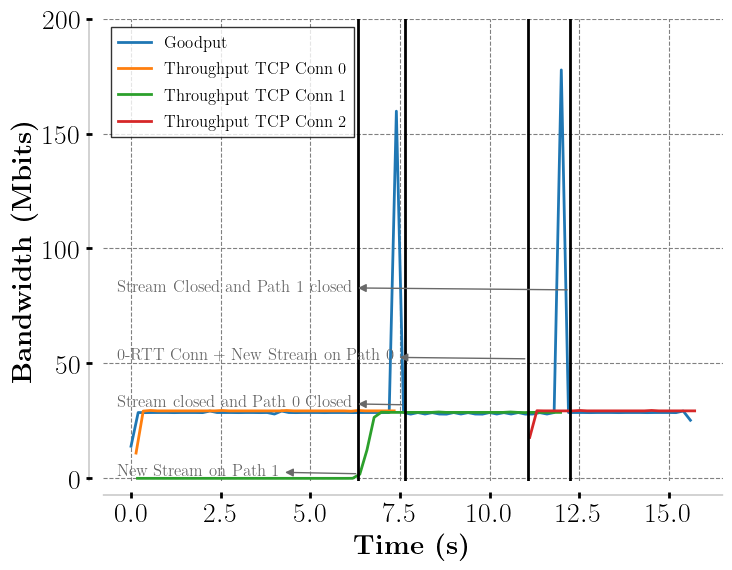
\includegraphics[width=.8\columnwidth]{figures/migration.png}
  \end{center}
\vspace{-0.5cm}
  \caption{Application-level connection migration during a 60MB file download.
    \tcpls temporarily aggregates the two network paths during such a migration.}
  \label{fig:conn_migration}
\end{figure}

\subsection{Dynamically Extending \tcpls}

The \tcpls streams enable new use case. Obviously, a \tcpls application can
create and use different streams to carry data. However, since these streams
are generic, they can also be used by the \tcpls implementation itself to
exchange control information. To demonstrate the versatily of these control
streams, we extended \tcpls to enable a server to push a different congestion
control scheme to a specific client over an existing \tcpls session. Recent
work on restructuring congestion control has proposed a generic architecture
for congestion controllers~\cite{narayan2018restructuring}.
During the last years, the Linux kernel developpers have relied on eBPF
to make the Linux TCP/IP stack~\cite{brakmo2017tcp,tran2020beyond} easier
to extend. Since Linux kernel version 5.6, an application can inject
a different congestion control scheme entirely implemented using eBPF. A similar
approach was proposed in Pluginizing \quic~\cite{de2019pluginizing}. We
leverage these new eBPF capabilities to demonstrate the feasibility of injecting
and updating a congestion control scheme during a \tcpls session.

We perform our experiment using Mininet over a 100Mbps emulated link
that has a 60msec delay. Fig.~\ref{fig:vegasCubic} shows a client that uses the \tcp Vegas~\cite{10.1145/190314.190317} congestion control scheme to upload a file. This \tcpls session fully uses the bottleneck link. After some time, another client starts an upload, but using the CUBIC congestion controller~\cite{rfc8312}. This results in an unfair distribution of the
bandwidth. The server then sends the eBPF bytecode implementing the CUBIC congestion control scheme to the \tcp Vegas client that injects it in its kernel and the unfairness disappears. We performed the same experiment for different delays, varying from 10ms to 100ms and obtained similar results.

\begin{figure}[!t]
  \begin{center}
    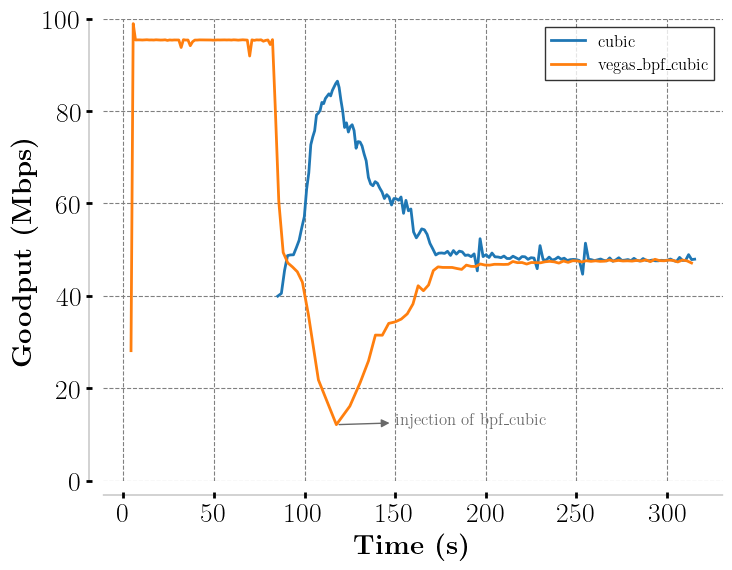
\includegraphics[width=.8\columnwidth]{pretty_plotify/plots/vegas_cubic.png}
  \end{center}
\vspace{-0.5cm}
  \caption{\tcpls hosts can exchange congestion control schemes compiled into eBPF bytecode and activate them during a \tcpls session.}
  \label{fig:vegasCubic}
\end{figure}
